



\section{Visualizacion de datos}

La visualización de datos es la práctica de traducir información en un contexto visual, como un mapa o gráfico, para facilitar que el cerebro humano comprenda y extraiga información útil.\\

Las formas más generales de visualización de datos son las siguientes: Gráficas, Tablas, Mapas, Infografias y Tableros. En este trabajo se hará uso especificamente de gráficas como medio de visualización de datos, ya que los datos obtenidos de Wikipedia no permiten ser visualizados de otra forma.


\subsection{Tipos de gráficas}

\section{Dominio del problema}
    \subsection{Wiki}

        El término wiki proviene de la raiz hawaiana wiki, que significa "rápido", y fue propuesto por Ward Cunningham, quien a su vez define los sitios web wiki como "La base de datos más simple que puede existir" [Cunningham, Ward (June 27, 2002), What is a Wiki]. Con el tiempo el concepto de Wiki fue evolucionando, y hoy en dia cuando hablamos de wiki nos referimos a un sitio web que permite a sus usuarios colaborar en su estructura y contenido.\\
        
        Wikimedia es el nombre colectivo del movimiento wikimedia, que incluye un grupo de proyectos interrelacionados, tales como: Wikipedia, Wiktionary, Wikiquote, Wikibooks, Wikisource, entre otros, cuyo proposito es usar el poder colaborativo de internet, y el concepto wiki, para compartir conocimiento gratuito de cualquier tipo.\\
        
        MediaWiki es el motor que impulsa los sitios web basados en wiki. En este documento se hará efasis en este sistema, debido a que se trabajará con articulos de Wikipedia, quien hace uso de Mediawiki para cumplir con muchas de sus funcionalidades.

    \subsection{Filosofía de la wiki}

        [https://www.um.es/ead/red/M11/intro.pdf]
        [https://ignasialcalde.es/filosofia-wiki-y-dinamicas-relacionales/]
        
        Antes de la existencia del internet, la información era poder, y saber mucho era tener mucha información. En esos tiempos la información era en su mayoria fisica y centralizada, lo que le otorgaba muchisimo valor. En la actualidad la información es considerada virtualmente ubicua y en constante cambio, y lo que realmente ofrece valor es la capacidad individual de sintetizar esa información y relacionarla, además de saber utilizar esa información con un fin.

        La filosofia de wiki surge con el proposito de 

    \subsection{Watcher}

    \subsection{Wikipedia como ejemplo práctico}

    \subsection{Visualizacion cientifica}


\subsection{Tecnologias a utilizar}

    Para la realización de este proyecto se usaran las siguientes tecnologias:

    \subsubsection{ReactJS}

        ReactJS es una librería de JavaScript de código abierto desarrollada por Facebook para facilitar la creación de componentes interactivos, reutilizables, para desarrollos de interfaces de usuario, especialmente aplicaciones de una sola página.

        React maneja el concepto de \say{programación reactiva} haciendo uso de un DOM Virtual, lo le permite determinar qué partes del DOM han cambiado comparando contenidos entre la versión nueva y la almacenada den el DOM virtual, para así propagar los datos generando cambios en la aplicación, es decir, los datos \say {reaccionan} ejecutando una serie de eventos.\\

        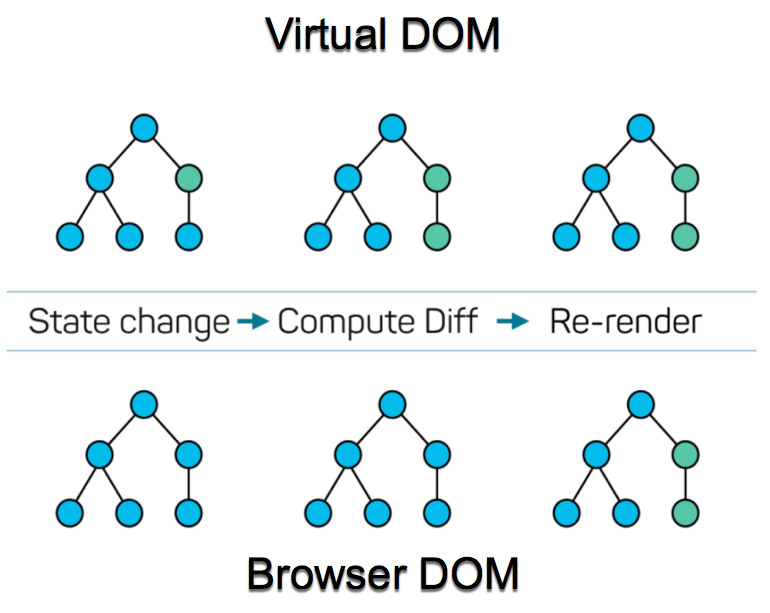
\includegraphics[scale=0.5]{virtual_dom}\\

        Este concepto de reactividad es lo que hace a la libreria altamente eficiente, ya que limita la actualización del DOM solamente a los elementos que han cambiado.
        
    \subsubsection{NextJS}
        NextJS es un framework desarrollado encima de Node.js que permite a las aplicaciones de React usar funcionalidades como el renderizado en la parte servidor 

    \subsubsection{SEO}
    
        Se trata del proceso de mejorar un sitio web en relación con los motores de búsqueda. También representa el cargo de la persona que trabaja en este proceso: Acabamos de contratar a un nuevo SEO para que mejore nuestra presencia en la Web.

    \subsubsection{Fastify}

    \subsubsection{Mongo}

        MongoDB es un sistema de base de datos NoSQL, orientado a documentos y de código abierto. En lugar de guardar los datos en tablas, tal y como se hace en las bases de datos relacionales, MongoDB guarda estructuras de datos BSON (una especificación similar a JSON) con un esquema dinámico, haciendo que la integración de los datos en ciertas aplicaciones sea más fácil y rápida.

        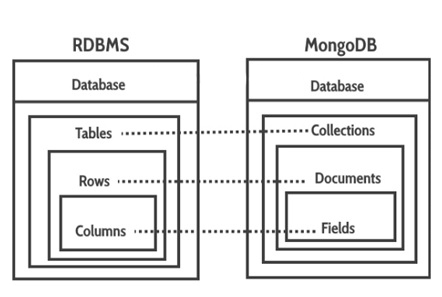
\includegraphics{mongodb-structure.jpg}


\subsection{Metodologias agiles}


    \subsubsection{Frameworks}

    \begin{enumerate}
        \item Kanban
        \item Scrum
        \item Extreme programming (XP)
        \item Dynamic systems development method (DSDM)
        \item Lean software development
        \item Adaptive Software Development (ASD):
        \item Rapid application development (RAD)
    \end{enumerate}

    \subsubsection{Prácticas}

    \begin{enumerate}
        \item Acceptance test-driven development (ATDD)
        \item Agile modeling
        \item Agile testing
        \item Backlogs (Product and Sprint)
        \item Behavior-driven development (BDD)
        \item Continuous integration (CI)
        \item Cross-functional team
        \item Daily Stand-up / Daily Scrum
        \item Domain-driven design (DDD)
        \item Iterative and incremental development (IID)
        \item Pair programming
        \item Planning poker
        \item Refactoring
        \item Retrospective
        \item Scrum events (sprint planning, sprint review and retrospective)
        \item Specification by example
        \item Story-driven modeling
        \item Test-driven development (TDD)
        \item Timeboxing
        \item User story
        \item Velocity tracking
    \end{enumerate}

